% Options for packages loaded elsewhere
\PassOptionsToPackage{unicode}{hyperref}
\PassOptionsToPackage{hyphens}{url}
%
\documentclass[
]{article}
\usepackage{lmodern}
\usepackage{amssymb,amsmath}
\usepackage{ifxetex,ifluatex}
\ifnum 0\ifxetex 1\fi\ifluatex 1\fi=0 % if pdftex
  \usepackage[T1]{fontenc}
  \usepackage[utf8]{inputenc}
  \usepackage{textcomp} % provide euro and other symbols
\else % if luatex or xetex
  \usepackage{unicode-math}
  \defaultfontfeatures{Scale=MatchLowercase}
  \defaultfontfeatures[\rmfamily]{Ligatures=TeX,Scale=1}
\fi
% Use upquote if available, for straight quotes in verbatim environments
\IfFileExists{upquote.sty}{\usepackage{upquote}}{}
\IfFileExists{microtype.sty}{% use microtype if available
  \usepackage[]{microtype}
  \UseMicrotypeSet[protrusion]{basicmath} % disable protrusion for tt fonts
}{}
\makeatletter
\@ifundefined{KOMAClassName}{% if non-KOMA class
  \IfFileExists{parskip.sty}{%
    \usepackage{parskip}
  }{% else
    \setlength{\parindent}{0pt}
    \setlength{\parskip}{6pt plus 2pt minus 1pt}}
}{% if KOMA class
  \KOMAoptions{parskip=half}}
\makeatother
\usepackage{xcolor}
\IfFileExists{xurl.sty}{\usepackage{xurl}}{} % add URL line breaks if available
\IfFileExists{bookmark.sty}{\usepackage{bookmark}}{\usepackage{hyperref}}
\hypersetup{
  pdftitle={Climate variability indices for ecological and crop models in R: the climatrends package},
  hidelinks,
  pdfcreator={LaTeX via pandoc}}
\urlstyle{same} % disable monospaced font for URLs
\usepackage[margin=1in]{geometry}
\usepackage{color}
\usepackage{fancyvrb}
\newcommand{\VerbBar}{|}
\newcommand{\VERB}{\Verb[commandchars=\\\{\}]}
\DefineVerbatimEnvironment{Highlighting}{Verbatim}{commandchars=\\\{\}}
% Add ',fontsize=\small' for more characters per line
\usepackage{framed}
\definecolor{shadecolor}{RGB}{248,248,248}
\newenvironment{Shaded}{\begin{snugshade}}{\end{snugshade}}
\newcommand{\AlertTok}[1]{\textcolor[rgb]{0.94,0.16,0.16}{#1}}
\newcommand{\AnnotationTok}[1]{\textcolor[rgb]{0.56,0.35,0.01}{\textbf{\textit{#1}}}}
\newcommand{\AttributeTok}[1]{\textcolor[rgb]{0.77,0.63,0.00}{#1}}
\newcommand{\BaseNTok}[1]{\textcolor[rgb]{0.00,0.00,0.81}{#1}}
\newcommand{\BuiltInTok}[1]{#1}
\newcommand{\CharTok}[1]{\textcolor[rgb]{0.31,0.60,0.02}{#1}}
\newcommand{\CommentTok}[1]{\textcolor[rgb]{0.56,0.35,0.01}{\textit{#1}}}
\newcommand{\CommentVarTok}[1]{\textcolor[rgb]{0.56,0.35,0.01}{\textbf{\textit{#1}}}}
\newcommand{\ConstantTok}[1]{\textcolor[rgb]{0.00,0.00,0.00}{#1}}
\newcommand{\ControlFlowTok}[1]{\textcolor[rgb]{0.13,0.29,0.53}{\textbf{#1}}}
\newcommand{\DataTypeTok}[1]{\textcolor[rgb]{0.13,0.29,0.53}{#1}}
\newcommand{\DecValTok}[1]{\textcolor[rgb]{0.00,0.00,0.81}{#1}}
\newcommand{\DocumentationTok}[1]{\textcolor[rgb]{0.56,0.35,0.01}{\textbf{\textit{#1}}}}
\newcommand{\ErrorTok}[1]{\textcolor[rgb]{0.64,0.00,0.00}{\textbf{#1}}}
\newcommand{\ExtensionTok}[1]{#1}
\newcommand{\FloatTok}[1]{\textcolor[rgb]{0.00,0.00,0.81}{#1}}
\newcommand{\FunctionTok}[1]{\textcolor[rgb]{0.00,0.00,0.00}{#1}}
\newcommand{\ImportTok}[1]{#1}
\newcommand{\InformationTok}[1]{\textcolor[rgb]{0.56,0.35,0.01}{\textbf{\textit{#1}}}}
\newcommand{\KeywordTok}[1]{\textcolor[rgb]{0.13,0.29,0.53}{\textbf{#1}}}
\newcommand{\NormalTok}[1]{#1}
\newcommand{\OperatorTok}[1]{\textcolor[rgb]{0.81,0.36,0.00}{\textbf{#1}}}
\newcommand{\OtherTok}[1]{\textcolor[rgb]{0.56,0.35,0.01}{#1}}
\newcommand{\PreprocessorTok}[1]{\textcolor[rgb]{0.56,0.35,0.01}{\textit{#1}}}
\newcommand{\RegionMarkerTok}[1]{#1}
\newcommand{\SpecialCharTok}[1]{\textcolor[rgb]{0.00,0.00,0.00}{#1}}
\newcommand{\SpecialStringTok}[1]{\textcolor[rgb]{0.31,0.60,0.02}{#1}}
\newcommand{\StringTok}[1]{\textcolor[rgb]{0.31,0.60,0.02}{#1}}
\newcommand{\VariableTok}[1]{\textcolor[rgb]{0.00,0.00,0.00}{#1}}
\newcommand{\VerbatimStringTok}[1]{\textcolor[rgb]{0.31,0.60,0.02}{#1}}
\newcommand{\WarningTok}[1]{\textcolor[rgb]{0.56,0.35,0.01}{\textbf{\textit{#1}}}}
\usepackage{graphicx}
\makeatletter
\def\maxwidth{\ifdim\Gin@nat@width>\linewidth\linewidth\else\Gin@nat@width\fi}
\def\maxheight{\ifdim\Gin@nat@height>\textheight\textheight\else\Gin@nat@height\fi}
\makeatother
% Scale images if necessary, so that they will not overflow the page
% margins by default, and it is still possible to overwrite the defaults
% using explicit options in \includegraphics[width, height, ...]{}
\setkeys{Gin}{width=\maxwidth,height=\maxheight,keepaspectratio}
% Set default figure placement to htbp
\makeatletter
\def\fps@figure{htbp}
\makeatother
\setlength{\emergencystretch}{3em} % prevent overfull lines
\providecommand{\tightlist}{%
  \setlength{\itemsep}{0pt}\setlength{\parskip}{0pt}}
\setcounter{secnumdepth}{-\maxdimen} % remove section numbering
\usepackage{caption} \captionsetup[figure]{labelformat=empty}
\usepackage{booktabs}
\usepackage{longtable}
\usepackage{array}
\usepackage{multirow}
\usepackage{wrapfig}
\usepackage{float}
\usepackage{colortbl}
\usepackage{pdflscape}
\usepackage{tabu}
\usepackage{threeparttable}
\usepackage{threeparttablex}
\usepackage[normalem]{ulem}
\usepackage{makecell}
\usepackage{xcolor}
\newlength{\cslhangindent}
\setlength{\cslhangindent}{1.5em}
\newenvironment{cslreferences}%
  {\setlength{\parindent}{0pt}%
  \everypar{\setlength{\hangindent}{\cslhangindent}}\ignorespaces}%
  {\par}

\title{Climate variability indices for ecological and crop models in R:
the \texttt{climatrends} package}
\author{}
\date{\vspace{-2.5em}25 May 2020}

\begin{document}
\maketitle

\begin{quote}
Kauê de Sousa\textsuperscript{1,2{[}*{]}}, Jacob van
Etten\textsuperscript{2}, Svein Øivind Solberg\textsuperscript{1}\\
\textsuperscript{1} Department of Agricultural Sciences, Inland Norway
University of Applied Sciences, 2318 Hamar, Norway\\
\textsuperscript{2} Bioversity International, 00054 Maccarese, Rome,
Italy\\
\textsuperscript{{[}*{]}}Correspondence should be addressed to:
\href{mailto:kaue.desousa@inn.no}{\nolinkurl{kaue.desousa@inn.no}}
\end{quote}

\hfill\break

\hypertarget{introduction}{%
\section{Introduction}\label{introduction}}

Abiotic factors plays an important role in most ecological and crop
systems that depends on certain levels of temperature, light and
precipitation (and their interplay) to initiate important physiological
events (Schulze et al. 2019). In the walk of climate change, understand
how these factors drives the physiological processes is a key approach
to provide recommendations for adaptation and biodiversity conservation.
If translated to stress

Raw temperature and precipitation values are \ldots{} to describe how
organisms interacts with the enviroment

\texttt{climatrends} aims to provide the R (R Core Team 2020) toolkit to
compute extreme precipitation and temperature indices that serves as
input for climate and crop models (van Etten et al. 2019; Kehel, Crossa,
and Reynolds 2016), trends in climate change (Aguilar et al. 2005; de
Sousa et al. 2018) and applied ecology (Prentice et al. 1992; Liu and
El-Kassaby 2018).

{[}\ldots continue\ldots{]}

\hypertarget{methods-and-features}{%
\section{Methods and features}\label{methods-and-features}}

\hypertarget{implementation}{%
\subsection{Implementation}\label{implementation}}

Six main functions are provided, \texttt{crop\_sensitive()},
\texttt{ETo()}, \texttt{GDD()}, \texttt{late\_frost()},
\texttt{rainfall()} and \texttt{temperature()} with a default method for
numeric `vector's and additional methods implemented via the package
\texttt{methods} (R Core Team 2020) for classes 'matrix' (or array),
`data.frame', and `sf' (of geometry POINT or POLYGON) (Pebesma 2018).
The later two are designed to fetch data from cloud sources.

say that the idea for the functions started with citizen science
projects that is why \texttt{day.one} and \texttt{span} may be variable
across locations. For time series analysis where fixed periods are
defined across many locations the indices can be adjusted with last.day.

{[}\ldots continue\ldots{]}

\hypertarget{temperature-and-precipitation-indices}{%
\subsection{Temperature and precipitation
indices}\label{temperature-and-precipitation-indices}}

\hypertarget{growing-degree-days}{%
\subsection{Growing degree-days}\label{growing-degree-days}}

Growing degree-days (gdd) is an heuristic tool in phenology that
measures heat accumulation and is used to predict plant and animal
development rates (Prentice et al. 1992). Growing degree-days are
calculated by taking the integral of warmth above a base temperature
(\(T_{0}\)). The function \texttt{GDD()} applies by default the
following equation.

Equation {[}1{]}

\[GDD = \frac{T_{max} + T_{min}}{2} - T_{0}\]

Where \(T_{max}\) is the maximum temperature in the given day,
\(T_{min}\) is the minimum temperature in the given day and \(T_{0}\) is
the minimum temperature for growth (as per the physiology of the focal
organism or ecosystem averages).

Additionally, the function \texttt{GDD()} offers three modified
equations designed for cold environments and for tropical environments.
For cold environments, where \(T_{min}\) may be lower than \(T_{0}\),
there are two modified equations that adjusts either \(T_{mean}\)
(variant a) or \(T_{min}\) (variant b). The variant a changes
\(T_{mean}\) to \(T_{0}\) if \(T_{mean} < T_{0}\) and is expressed as
follows.

Equation {[}2{]}

\[ GDD = max \left(\frac{T_{max} + T_{min}}{2} - T_{0}, \; 0 \right)\]

The variant b, is calculated using Equation 1, but adjusts \(T_{min}\)
or \(T_{max}\) to \(T_{0}\) if \(T < T_{0}\), the equation is adjusted
as follows.

Equation {[}3{]}

\[ T < T_{0} \; \rightarrow \; T = T_{0} \]

Where \(T\) may refer to \(T_{min}\) and/or \(T_{max}\) when the
condition of being below \(T_{0}\) applies.

For tropical areas, where the temperature may surpass a maximum
threshold (\(T_{0^{max}}\)), resulting in limited development, the
minimum temperature is adjusted using Equation 3 and the maximum
temperature is adjusted to a maximum base temperature as follow.

Equation {[}4{]}

\[ T_{max} > T_{0^{max}} \; \rightarrow \; T_{max} = T_{0^{max}} \]

Where \(T_{0^{max}}\) is the maximum base temperature for growth,
defined in \texttt{GDD()} using the argument \texttt{tbase\_max}.

These modified equations are defined as `a', `b' and `c', respectively,
and can be selected using the argument \texttt{equation}.

By default, the function returns the degree-days that is accumulated
over the time series using Equation 1. Additionally, the function may
return the daily values of degree-days or the number of days that a
given organism required to reach a certain number of accumulated
degree-days. These values are defined by `acc', `daily' or `ndays' and
can be adjusted using the argument \texttt{return.as}. The required
accumulated gdd is defined with argument \texttt{degree.days}. For
example, the Korean pine (\emph{Pinus koraiensis}) requires 105
\(^\circ C\) accumulated gdd to onset the photosynthesis (Wu et al.
2013). In that case, \texttt{GDD()} will calculate the growing
degree-days (\(gdd\)) and sum up the values until it reaches 105
\(^\circ C\) and return the number of days required in the given season
(\(GDD_{r}\)), as follows.

Equation {[}5{]}

\[\parallel GDD_{r} \parallel \: = \; ggd_1 \;+ \; ...  \; +  \; gdd_n\]

\hypertarget{late-spring-frost}{%
\subsection{Late-spring frost}\label{late-spring-frost}}

\hypertarget{crop-related-indices}{%
\subsection{Crop-related indices}\label{crop-related-indices}}

Two functions in \textbf{climatrends} are mainly designed to capture the
effects of climate on the development and stress of crop species,
\texttt{crop\_sensitive} computes indices that aims to capture the
changes in temperature extremes during key phenological stages
(e.g.~anthesis), and \texttt{ETo()} computes the reference
evapotranspiration.

The reference evapotranspiration measures the influence of the climate
on a given organism water needs, generally a crop species (Brouwer and
Heibloem 1986). The function \texttt{ETo()} applies the Blaney-Criddle
method, a general theoretical method used when only air-temperature is
available locally. It should be noted that this method is not very
accurate and aims to provide the order of magnitude of
evapotranspitation. The reference evapotranspiration is calculated using
the following equation.

Equation {[}6{]}

\[ETo = p \times \left(0.46 \times \frac{T_{max} + T_{min}}{2} + 8 \right) \times K_c\]

Where \(p\) is the mean daily percentage of annual daytime hours,
\(T_{max}\) is the maximum temperature, \(T_{min}\) is the minimum
temperature, and \(K_c\) is the factor for organism water need.

The percentage of daytime hours (\(p\)) is calculated internally by the
`data.frame' and `sf' methods in \texttt{ETo()} using the given latitude
(taken from the inputted \texttt{object}) and date (taken from the
inputted \texttt{day.one}). It matches the latitude and date with a
table of daylight percentage derived from Brouwer and Heibloem (1986).
The table can be verified using \texttt{climatrends:::daylight}.

\hypertarget{examples}{%
\section{Examples}\label{examples}}

\hypertarget{seed-germination-or-some-gdd-related-analysis}{%
\subsection{Seed germination or some GDD related
analysis}\label{seed-germination-or-some-gdd-related-analysis}}

Use the data from seed germination or crop growth to compute GDD. How
many GDD a seed need to become a seedling?

\hypertarget{common-beans}{%
\subsection{Common beans}\label{common-beans}}

During five growing seasons (from 2015 to 2016 in Nicaragua), van Etten
et al (2019) conducted a crowdsourcing citizen-science trial testing 11
common beans varieties (\emph{Phaseolus vulgaris} L.) in 842
farmer-managed experimental plots. Sets of three varieties were
allocated randomly to farms as incomplete blocks, maintaining spatial
balance by assigning roughly equal frequencies of the varieties to each
area. For the analysis the authors applied the Plackett--Luce model,
which estimates for each variety the probability that it wins, beating
all other varieties in the set (Turner et al. 2020). The research showed
that this approach can register known specific effects of climate
variation on crop varietal performance. An earlier version of
\texttt{climatrends} was used in this research to capture the seasonal
climate variation, here we replicate part of this analysis in the matter
that concerns the calculation and application of the climate indices.

Is important to mention that this analysis shaped the implementation of
the methods \texttt{temperature.array()} and \texttt{rainfall.matrix()}.

\begin{Shaded}
\begin{Highlighting}[]
\KeywordTok{library}\NormalTok{(}\StringTok{"climatrends"}\NormalTok{)}
\KeywordTok{library}\NormalTok{(}\StringTok{"PlackettLuce"}\NormalTok{)}
\KeywordTok{library}\NormalTok{(}\StringTok{"tidyverse"}\NormalTok{)}

\CommentTok{\# compute the number of days required to accumulate}
\CommentTok{\# gdd from planting date to maturity}
\NormalTok{gdd <{-}}\StringTok{ }\KeywordTok{GDD}\NormalTok{(modis, }
           \DataTypeTok{day.one =}\NormalTok{ cbean}\OperatorTok{$}\NormalTok{planting\_date, }
           \DataTypeTok{degree.days =} \DecValTok{900}\NormalTok{, }
           \DataTypeTok{return.as =} \StringTok{"ndays"}\NormalTok{)}

\CommentTok{\# add gdd to the cbean data and take the average }
\CommentTok{\# of gdd per season}
\NormalTok{cbean }\OperatorTok{\%<>\%}\StringTok{  }
\StringTok{  }\KeywordTok{mutate}\NormalTok{(}\DataTypeTok{gdd =}\NormalTok{ gdd}\OperatorTok{$}\NormalTok{gdd) }\OperatorTok{\%>\%}\StringTok{ }
\StringTok{  }\KeywordTok{group\_by}\NormalTok{(season) }\OperatorTok{\%>\%}\StringTok{ }
\StringTok{  }\KeywordTok{mutate}\NormalTok{(}\DataTypeTok{gdds =} \KeywordTok{as.integer}\NormalTok{(}\KeywordTok{mean}\NormalTok{(gdd)))}
\end{Highlighting}
\end{Shaded}

\begin{Shaded}
\begin{Highlighting}[]
\CommentTok{\# compute the temperature indices from planting date to the }
\CommentTok{\# number of days required to accumulate the gdd in each season}
\NormalTok{temp <{-}}\StringTok{ }\KeywordTok{temperature}\NormalTok{(modis, }
                    \DataTypeTok{day.one =}\NormalTok{ cbean}\OperatorTok{$}\NormalTok{planting\_date, }
                    \DataTypeTok{span =}\NormalTok{ cbean}\OperatorTok{$}\NormalTok{gdds)}

\CommentTok{\# combine the indices with the main data}
\NormalTok{cbean <{-}}\StringTok{ }\KeywordTok{cbind}\NormalTok{(cbean, temp)}

\CommentTok{\# fit a Plackett{-}Luce tree}
\NormalTok{plt <{-}}\StringTok{ }\KeywordTok{pltree}\NormalTok{(G }\OperatorTok{\textasciitilde{}}\StringTok{ }\NormalTok{maxNT, }\DataTypeTok{data =}\NormalTok{ cbean, }\DataTypeTok{minsize =} \DecValTok{200}\NormalTok{)}
\end{Highlighting}
\end{Shaded}

\hypertarget{time-series}{%
\subsection{Time series}\label{time-series}}

Pick some random points in Norway (or Scandinavia??) and check how the
trends on temperature indices over the last 20 years.

\hypertarget{further-development}{%
\section{Further development}\label{further-development}}

Integration with other datasets as they become available in \texttt{R}
via API client packages. New indices related to the physiology of crops
to be implemented while I work on the rice data.

\hypertarget{acknowledgements}{%
\section{Acknowledgements}\label{acknowledgements}}

This work was supported by The Nordic Joint Committee for Agricultural
and Food Research (grant num. 202100-2817).

\hypertarget{authors-contributions}{%
\section{Authors' contributions}\label{authors-contributions}}

KdS and JvE conceived the ideas of implementing an \texttt{R} package.
JvE and SØS assisted in the implementation of methods. KdS wrote and
documented the software. {[}add other contributions\ldots{]}

\hypertarget{data-availability-statement}{%
\section{Data availability
statement}\label{data-availability-statement}}

The source code has been archived at {[}\textbf{add link}{]} as
\texttt{climatrends} version \textbf{X.Y.Z}. To explore the latest
functionalities of \texttt{climatrends}, please check the package's
updates at CRAN (\url{https://cran.r-project.org/package=climatrends}).

\hypertarget{references}{%
\section{References}\label{references}}

\hypertarget{refs}{}
\begin{cslreferences}
\leavevmode\hypertarget{ref-Aguilar2005}{}%
Aguilar, E., T. C. Peterson, P. Ramírez Obando, R. Frutos, J. A. Retana,
M. Solera, J. Soley, et al. 2005. ``Changes in precipitation and
temperature extremes in Central America and northern South America,
1961--2003.'' \emph{Journal of Geophysical Research} 110 (D23): D23107.
\url{https://doi.org/10.1029/2005JD006119}.

\leavevmode\hypertarget{ref-Brouwer1986}{}%
Brouwer, C., and M. Heibloem. 1986. \emph{Irrigation water management:
Irrigation water needs}. Training m. Rome, Italy: Food; Agriculture
Organization of The United Nations.
\url{http://www.fao.org/3/S2022E/s2022e00.htm}.

\leavevmode\hypertarget{ref-deSousa2018}{}%
de Sousa, Kauê, Fernando Casanoves, Jorge Sellare, Alejandra Ospina,
Jose Gabriel Suchini, Amilcar Aguilar, and Leida Mercado. 2018. ``How
climate awareness influences farmers' adaptation decisions in Central
America?'' \emph{Journal of Rural Studies} 64: 11--19.
\url{https://doi.org/10.1016/j.jrurstud.2018.09.018}.

\leavevmode\hypertarget{ref-Kehel2016}{}%
Kehel, Z., J. Crossa, and M. Reynolds. 2016. ``Identifying Climate
Patterns during the Crop-Growing Cycle from 30 Years of CIMMYT Elite
Spring Wheat International Yield Trials.'' In \emph{Applied Mathematics
and Omics to Assess Crop Genetic Resources for Climate Change Adaptive
Traits}, edited by Abdallah Bari, Ardeshir B. Damania, Michael Mackay,
and Selvadurai Dayanandan, 151--74. CRC Press.

\leavevmode\hypertarget{ref-YLiu2018}{}%
Liu, Yang, and Yousry A. El-Kassaby. 2018. ``Evapotranspiration and
favorable growing degree-days are key to tree height growth and
ecosystem functioning: Meta-analyses of Pacific Northwest historical
data.'' \emph{Scientific Reports} 8228 (October).
\url{https://doi.org/10.1038/s41598-018-26681-1}.

\leavevmode\hypertarget{ref-sf}{}%
Pebesma, Edzer. 2018. ``Simple Features for R: Standardized Support for
Spatial Vector Data.'' \emph{The R Journal} 10 (1): 439--46.
\url{https://doi.org/10.32614/RJ-2018-009}.

\leavevmode\hypertarget{ref-Prentice1992}{}%
Prentice, I. Colin, Wolfgang Cramer, Sandy P. Harrison, Rik Leemans,
Robert A. Monserud, and Allen M. Solomon. 1992. ``Special Paper: A
Global Biome Model Based on Plant Physiology and Dominance, Soil
Properties and Climate.'' \emph{Journal of Biogeography} 19 (2): 117.
\url{https://doi.org/10.2307/2845499}.

\leavevmode\hypertarget{ref-RCoreTeam}{}%
R Core Team. 2020. ``R: A language and environment for statistical
computing. version 4.0.0.'' Vienna, Austria: CRAN R Project.
\url{https://www.r-project.org/}.

\leavevmode\hypertarget{ref-PlantEcology}{}%
Schulze, Ernst-Detlef, Erwin Beck, Nina Buchmann, Stephan Clemens, Klaus
Müller-Hohenstein, and Michael Scherer-Lorenzen. 2019. \emph{Plant
Ecology}. Second Edi. Berlin, Germany: Springer.
\url{https://doi.org/10.1007/978-3-662-56233-8}.

\leavevmode\hypertarget{ref-Turner2020}{}%
Turner, Heather L, Jacob van Etten, David Firth, and Ioannis Kosmidis.
2020. ``Modelling rankings in R: the PlackettLuce package.''
\emph{Computational Statistics}.
\url{https://doi.org/10.1007/s00180-020-00959-3}.

\leavevmode\hypertarget{ref-vanEtten2019}{}%
van Etten, Jacob, Kauê de Sousa, Amílcar Aguilar, Mirna Barrios, Allan
Coto, Matteo Dell'Acqua, Carlo Fadda, et al. 2019. ``Crop variety
management for climate adaptation supported by citizen science.''
\emph{Proceedings of the National Academy of Sciences} 116 (10):
4194--9. \url{https://doi.org/10.1073/pnas.1813720116}.

\leavevmode\hypertarget{ref-JWu2013}{}%
Wu, Jiabing, Dexin Guan, Fenhui Yuan, Anzhi Wang, and Changjie Jin.
2013. ``Soil Temperature Triggers the Onset of Photosynthesis in Korean
Pine.'' Edited by Carl J. Bernacchi. \emph{PLoS ONE} 8 (6): e65401.
\url{https://doi.org/10.1371/journal.pone.0065401}.
\end{cslreferences}

\pagebreak

\hypertarget{figures-and-tables}{%
\section{Figures and tables}\label{figures-and-tables}}

\begin{table}

\caption{\label{tab:table1}Main functions available in climatrends.}
\centering
\resizebox{\linewidth}{!}{
\begin{tabular}[t]{l|>{\raggedright\arraybackslash}p{1in}|l|>{}p{1.7in}}
\hline
Name & Function & Output\\
\hline
crop\_sensitive() & Compute crop sensitive indices & A data frame with crop sensitive indices with n columns depending on the number of thresholds passed to each index\\
\hline
Eto() & Reference evapotranspiration & The reference evapotranspiration\\
\hline
GDD() & Compute growing degree-days & Either the cumulative sum of gdd across time (the default), or the gdd obtained in each day, or the number of days required to reach a certain amount of gdd\\
\hline
late\_frost() & Compute the occurrence of late-spring frost & A data.frame with the duration and gdd accumulated during the events of frost, latency (where there is no frost event, but also there is no gdd), and warming (where gdd is accumulated)\\
\hline
rainfall() & Precipitation indices & Either the indices considering the series as a whole, or time series indices splitted into equal intervals of days\\
\hline
temperature() & Temperature indices & Either the indices considering the series as a whole, or time series indices splitted into equal intervals of days\\
\hline
\end{tabular}}
\end{table}

\pagebreak

\begin{figure}
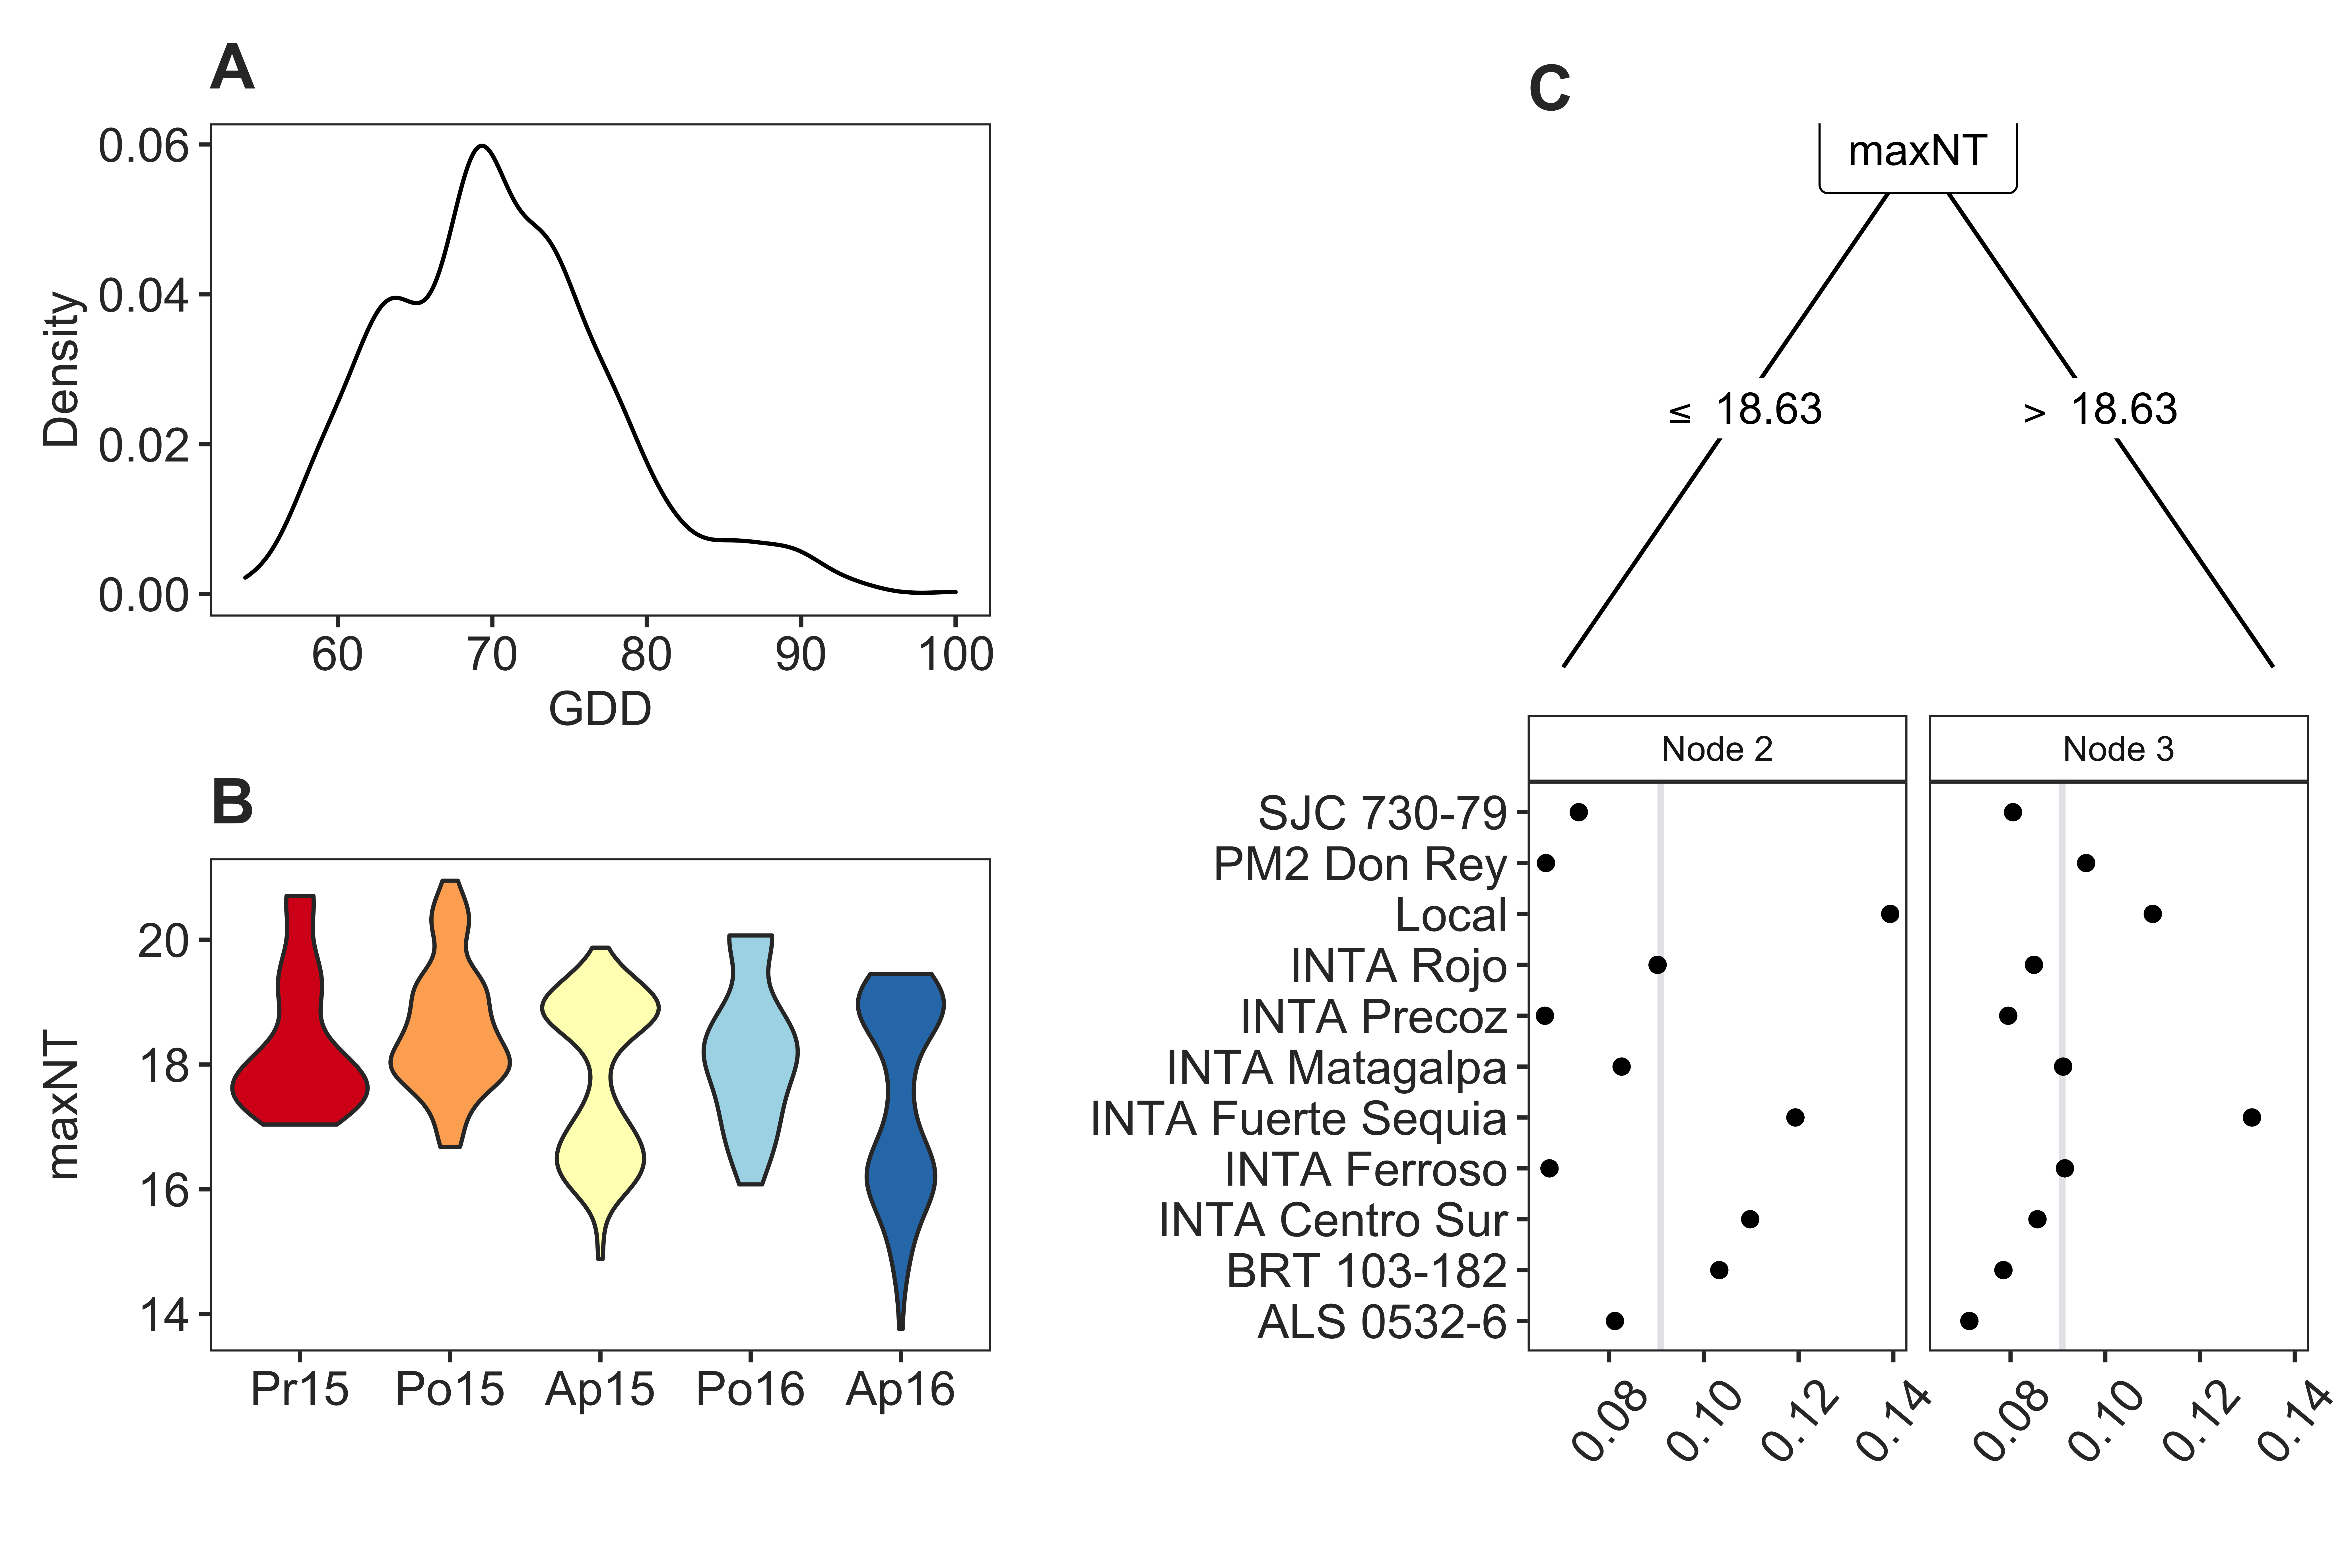
\includegraphics[width=0.8\linewidth]{cbean} \caption{Fig. 1. Application of climatrends functions to support the analysis of a citizen-science data testing 11 common bean varieties in Nicaragua. (A) Days required to reach 900 growing-degree days from planting date calculated using the function GDD(). (B) Maximum night temperature (°C) distributed across seasons computed using the function temperature(). (C) Plackett-Luce Tree showing the probability of one common bean variety has to win against the others (axys X) in two different nodes splitted with the maximum night temperature (°C).}\label{fig:fig_cbean}
\end{figure}

\end{document}
